
\chapter{Cellular automata}

%Nejaka citacia od Feynmana o CA, neznali CA budu prekvapeni: \cite{Andel07}

Years before DNA and replication mechanism was discovered in living cells,
John von Neumann was investigating self-replicating systems in theory, 
and layed basis for the "New kind of science" \cite{wolfram}. 

%It seems that there is some truth in this statement. One search of "cellular automata" on Arxiv outputs thousands of articles on application and theory of cellular automata only from recent years.

%However, for many colleague-scientist remain cellular automata "velkou neznamou".
%What the essence of cellular automata can be easily explained on the following famous example.

\section{Game of Life}

John Conway, by significant simplification of von Neumann ideas, introduced the Game of Life in 1970 that renewed general interest in cellular automata.

Depending on the initial conditions, evolution of this automaton can be chaotic, periodic or it can lead to the stable configurations.

The reason for this complexity hides in the fundamental property of Game of Life - because it is the Turing-complete, in principle any computer program can be simulated in the Game of Life, and thus any behavior can be observed.

For the purposes of this thesis, we have written a simple desktop application implementing this game, since we can easily explain the basic principles of cellular automata on it.

Let us have a rectangular grid, with black and white squares. 
White squares represent dead cells, black cells represent living cells.
On the figure \ref{gol1} we see such grid, that we chose for the initial state of 'Life'.


\begin{figure}[htbp]
 \centering
 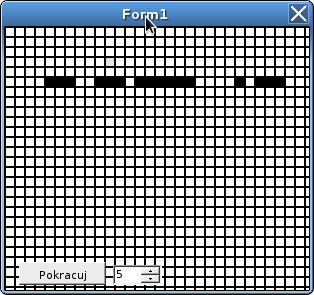
\includegraphics[width=0.7\textwidth]{./img/gol1}
 \label{gol1}
 \caption{The initial state of 'Life' (at t=0)}
\end{figure}

%The evolution of grid for our particular initial state is shown in figure blabla.\\  


\begin{figure}
 \centering
 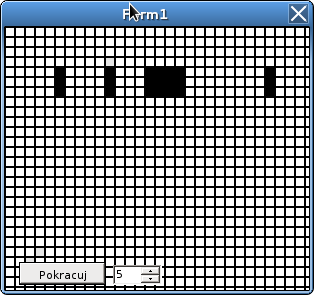
\includegraphics[width=0.7\textwidth]{./img/gol2}
 \label{gol2}
 \caption{t=1}
\end{figure}

\begin{figure}
 \centering
 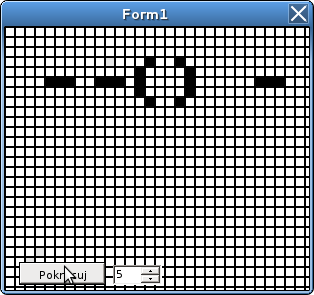
\includegraphics[width=0.7\textwidth]{./img/gol3}
 \label{gol2}
 \caption{t=2}
\end{figure}

Now we press 'Pokracuj' button and let the the Life evolve.
In the discrete time steps, the grid is changing.
We see that some cells are dying, but some cells are getting alive. 
What is the rule that kills the cell or leave it be? 

\begin{enumerate}
\item If the cell is alive, and 2 or 3 neighbouring cells are alive, the cell will stay alive in the next step. Otherwise it will die.
\item If the cell is dead, and \textbf{exactly} 3 neighboring cells are alive, the cell will get alive in the next step. Otherwise, it stays dead.

\end{enumerate}
We see that the rule involves only the state of \textbf{the cell} and the states of \textbf{its eight neighboring cells}.

\bigskip

Let us proceed from this simple example to a more general setting.
In the next section, we will generalize main features of 'Life' and formally define the cellular automaton.
%In the next chapter, we will generalize main feature of 'Life'
%Let us generalize this example into formal definition of cellular automaton.

\section{Cellular automaton in general}

\begin{enumerate}
\item \textbf{Position of the cells:}

Instead of two dimensional, rectangular grid of 'Life',
cells might be arranged on the regular grid of arbitrary dimensional. 
(Regularity follows from definition of Kubrid. In general, cells might be positioned really wildly,
e.g. on Penrose lattice, or arbritrary as proposed by Feynman).

\item \textbf{Set of cell states Q:}

In 'Life' cells can be dead or alive, but generally, set of states $Q$ for the cell can have an arbitrary finite size.
\bigskip

\item \textbf{Neighborhood:}

In 'Life', state of the cell in the next step was determined
by the nearest neighboring cells. We call these cells neighborhood of range r = 1 (in the distance of 1 cell).
However, the rule might involve neighborhood with the arbitrary range, see figure \ref{neighbor}

\begin{figure}
 \centering
 \includegraphics[width=1\textwidth]{./img/neighb}
 \label{neighbor}
 \caption{Moore's and von Neumann's neighborhood}
\end{figure}


\item \textbf{Update rule:}

Update rule is an arbitrary bounded mapping from the $neighborhood$ to the set of states $Q$.
Since the state of the cell is determined only by the state of its neighborhood, update rules in cellular automata are local.

\section{The most basic cellular automaton} 

In middle 1980s on the prestigious Princeton institute,
Stephen Wolfram and his assistants were performing unusual computer experiments. They were simulating the evolution of the one dimensional cellular automata and they were analyzing the obtained patterns \cite{levy} (to a despair of their senior colleagues, who did not understand this "new kind of science")\cite{wolfram}.

The most basic, one dimensional cellular automaton we can imagine, is the two state automaton with range $r=1$.

One dimensional indicates that the cells are arranged in the row (figure \ref{1d}), range $r=1$ indicates that the update rule involves only three cells.
An example of an update rule is shown the table~\ref{rule90}.

\begin{figure}[htbp]
 \centering 
 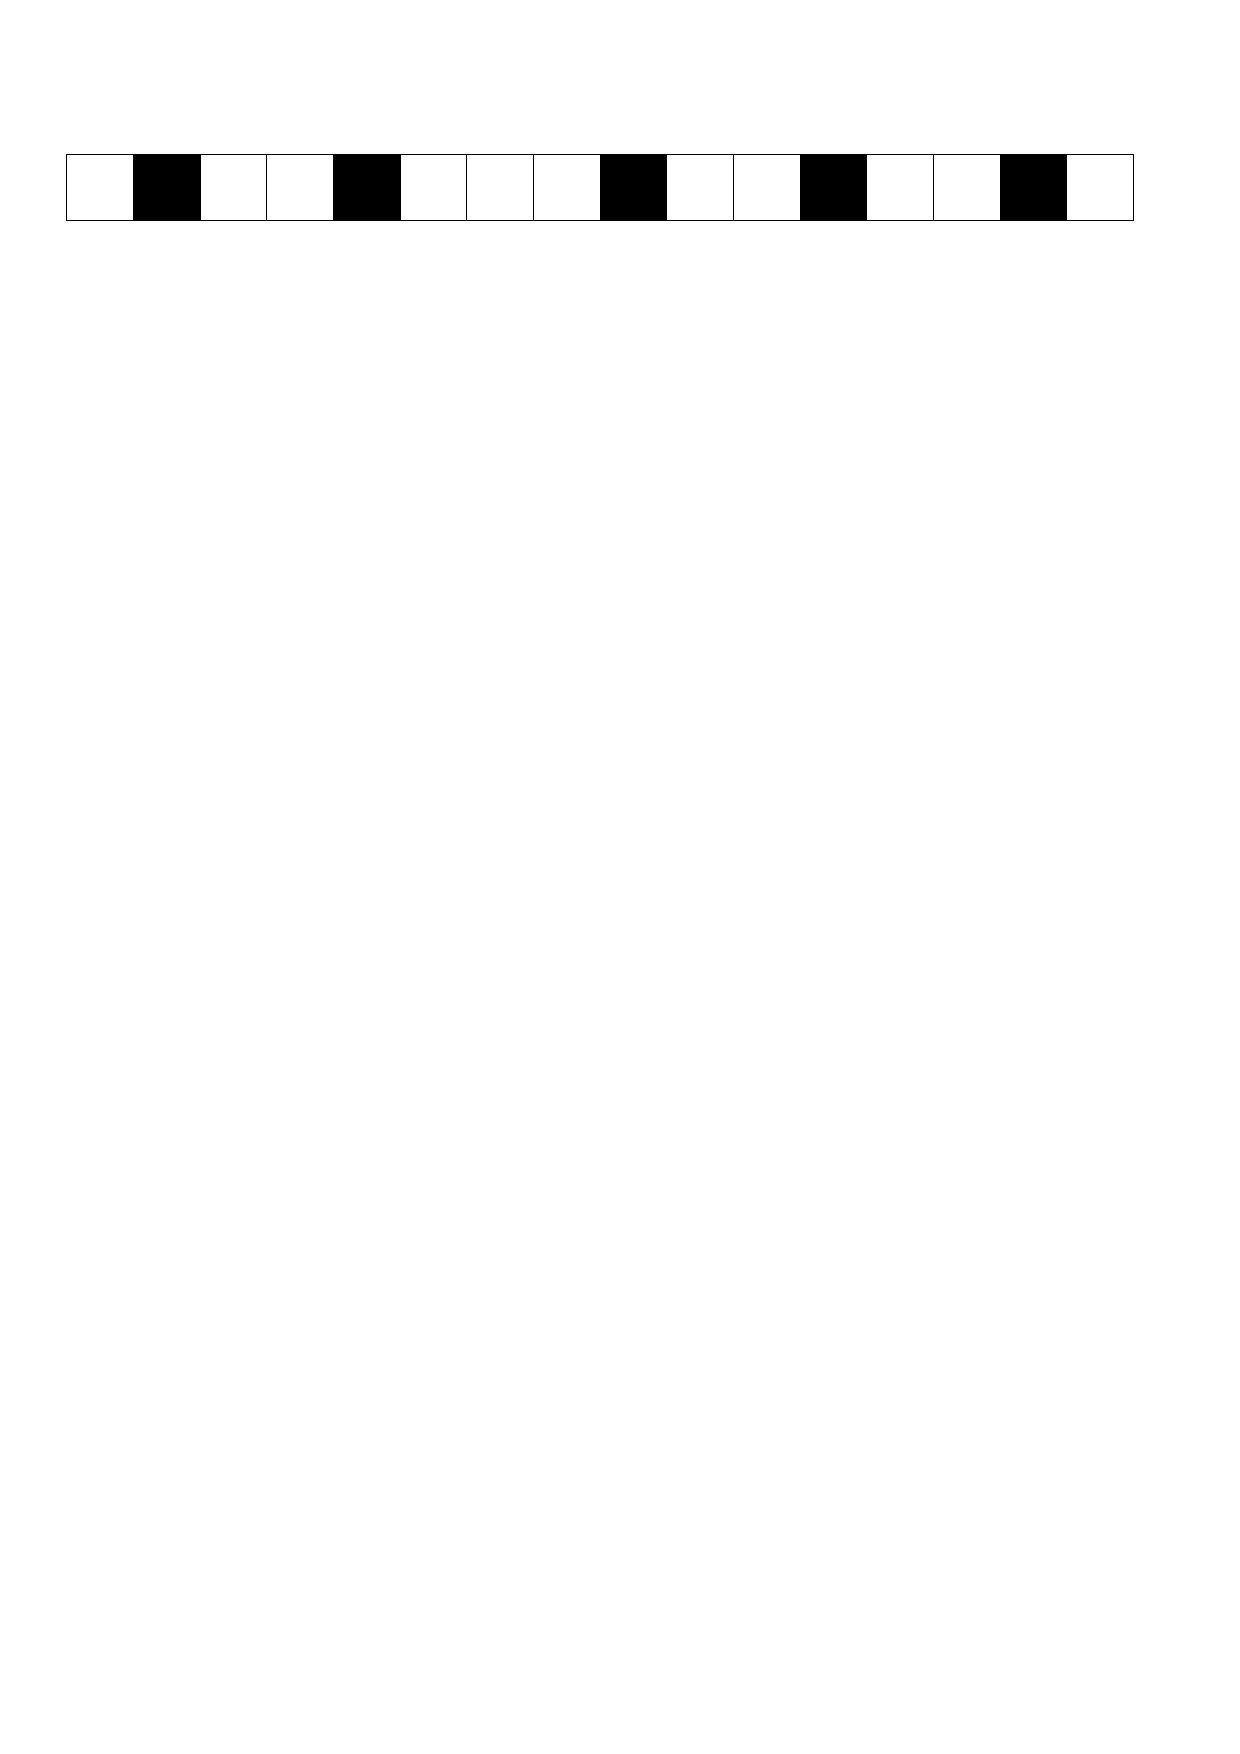
\includegraphics[width=0.9\textwidth]{./img/1Dline}
 \label{1d}
 \caption{A state of one dimensional cellular automaton}
\end{figure}


\begin{table}[htbp]
 \centering
 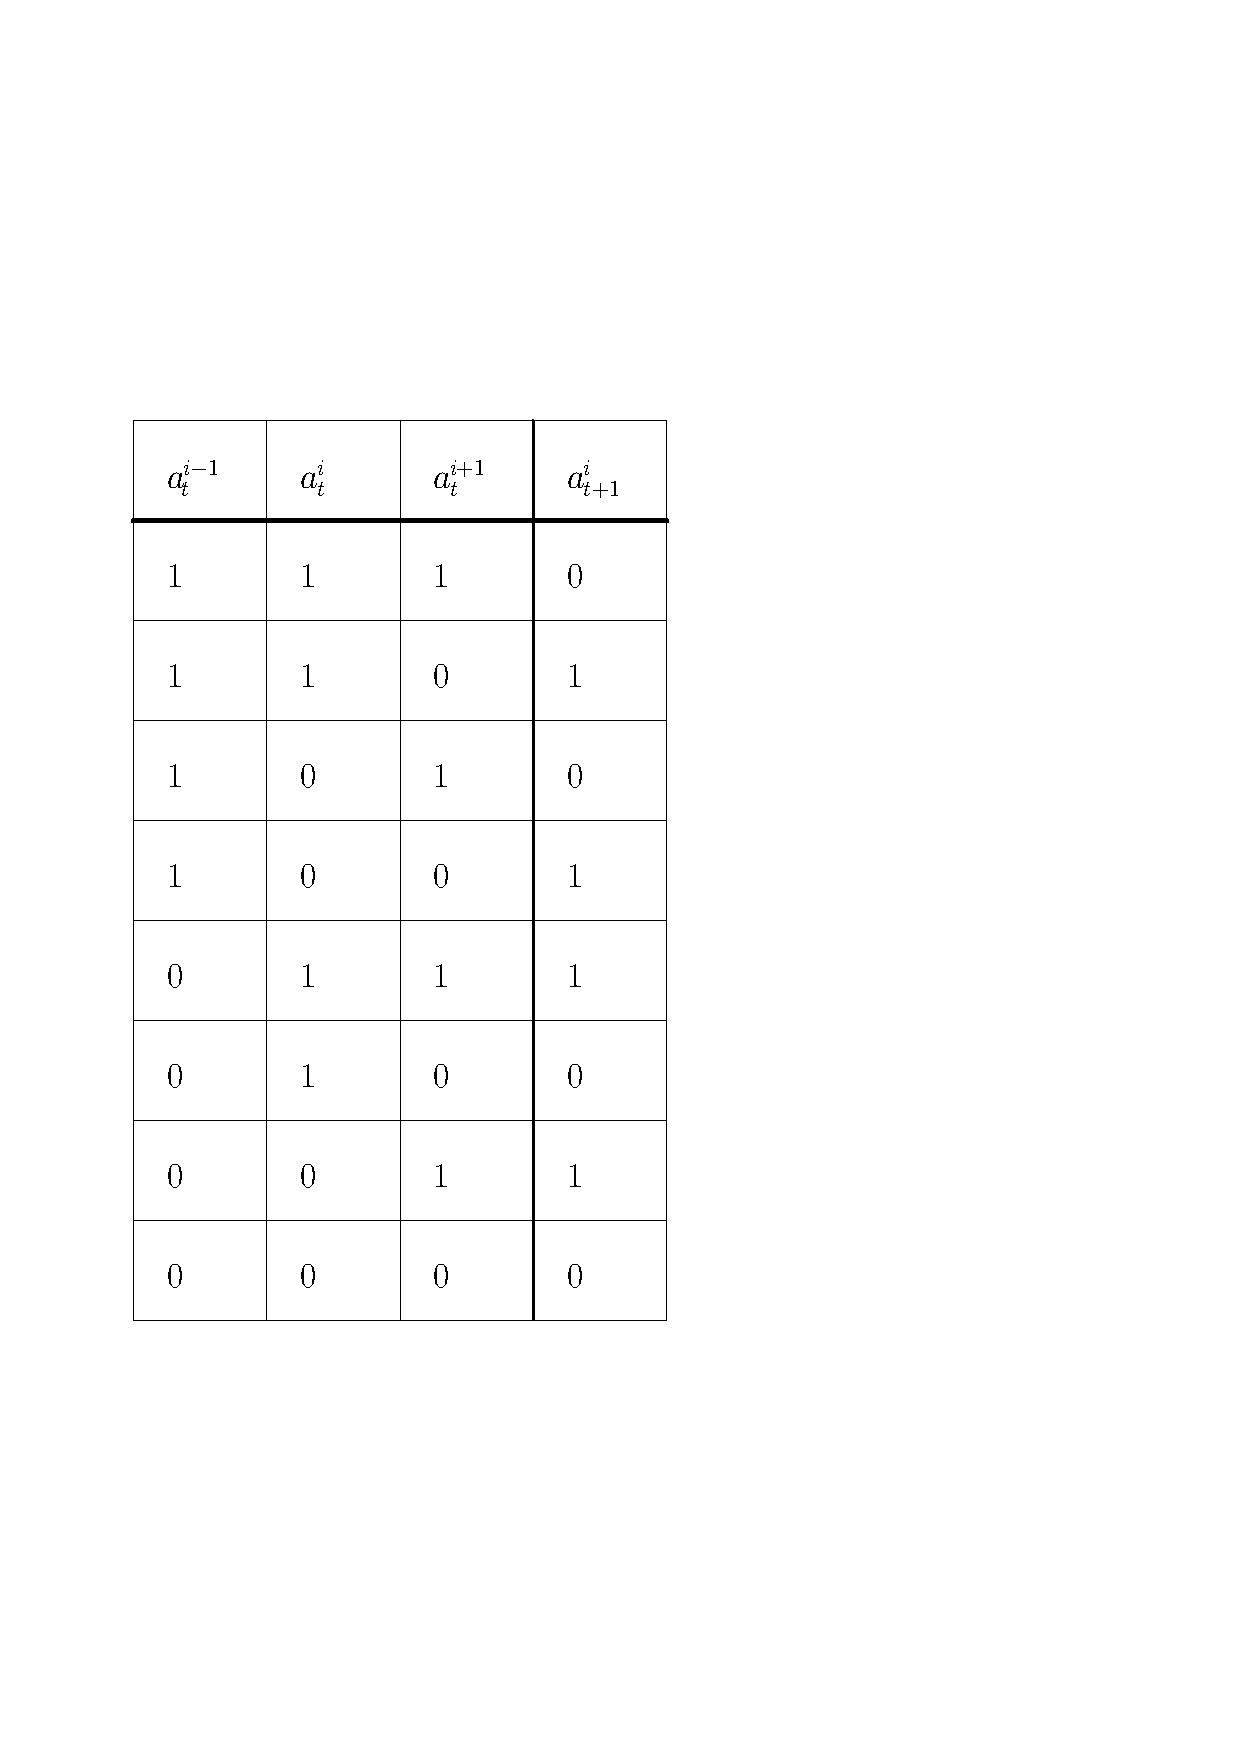
\includegraphics[width=0.4\textwidth]{./img/1Drule}
 \caption{Rule 90}
 \label{rule90}
\end{table}


The three columns represent the state of a cell $a_t^i$ and its left and right neighbor, $a_t^{i-1}$ and $a_t^{i+1}$ respectively. A living cell is denoted by 1, a dead cell is denoted by 0. The last column denotes the state of the middle cell $a_i$ in the next step $t+1$. The sequence of $one$s and $zero$s in the last column is the binary representation of a rule. In this particular case, of the Rule 90.
Since there is $2^8=256$ combinations for the last columns, there is $256$ rules for this most basic cellular automaton.

According to Wofram \cite{wolf}, these automata can be classified by their correspondence to the dynamical systems into three classes \cite{wolf}
\begin{enumerate}
\item \textbf{Limit point:}

The final configuration is homogeneous. 

Rules number $0,4,16,32,36,48,54,60,62$.

\item \textbf{Limit cycles:}

Simpe time-periodic patterns. 

Rules number $8,24,40,56,58$.

\item \textbf{Strange attractors:}

Chaotic patterns, see the figure \ref{rule30}. 

Rules number $2,6,10,12,14,18,22,26,28,30,34,38,42,44,46,50$.

%
%\item \textbf{No analogy to dynamical systems:}
%
%Rules number $20,52$.
%
\end{enumerate}

The figures were plotted by our own implementation of this automaton.
They represent the evolution of cellular automata with some of the mentioned rules.
The downer-most row is the initial configuration of the cellular automaton with one cell alive in the middle, all other cells are dead.
The $2^{nd}$ row is the configuration after the $1^{st}$ update and so forth.

Formally, the update rule that we have described by the table, may be written in the form
%The alternative formulation of the update rule that we just described can be written as \cite{wolf}
\begin{align} \label{rule1}
a_i^{(t)} = f \big[ \sum_{j=-r}^{j=r} \alpha_j a_{i+j}^{(t-1)} \big]
\end{align}
where $a_i$ refer to the state of the $j^{th}$ cell, $\alpha$s are the integer weights, and $f$ is the function that takes integer as the single argument, and $r$ is the range of the neighborhood.
\end{enumerate}

\begin{figure}[!t]
 \centering
 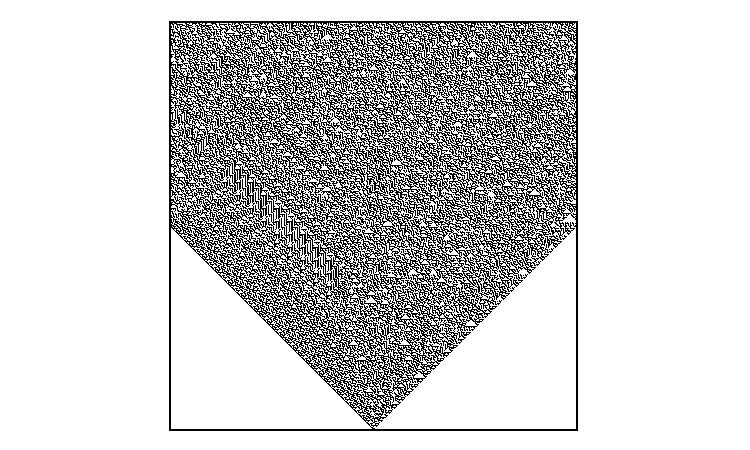
\includegraphics[trim = 40mm 0mm 0mm 0mm, width=1.7\textwidth]{./img/30_500}
 \caption{Rule 30}
 \label{rule30}
\end{figure}

\begin{figure}[!b]
 \centering
 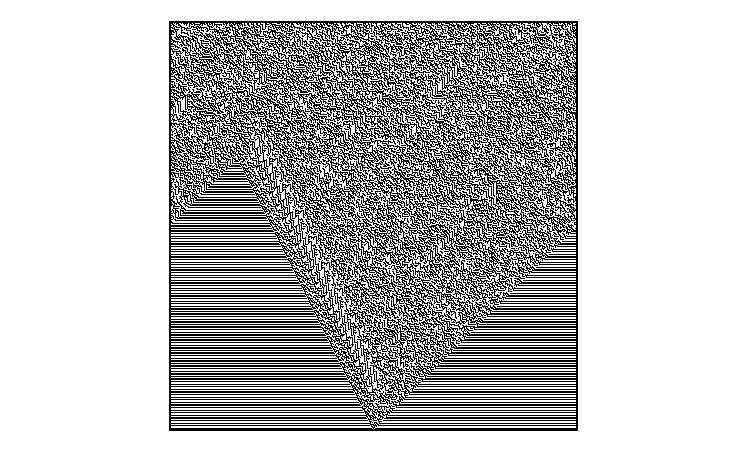
\includegraphics[trim = 40mm 0mm 0mm 0mm, width=1.7\textwidth]{./img/45_500}
 \caption{Rule 45}
\end{figure}

\begin{figure}
 \centering
 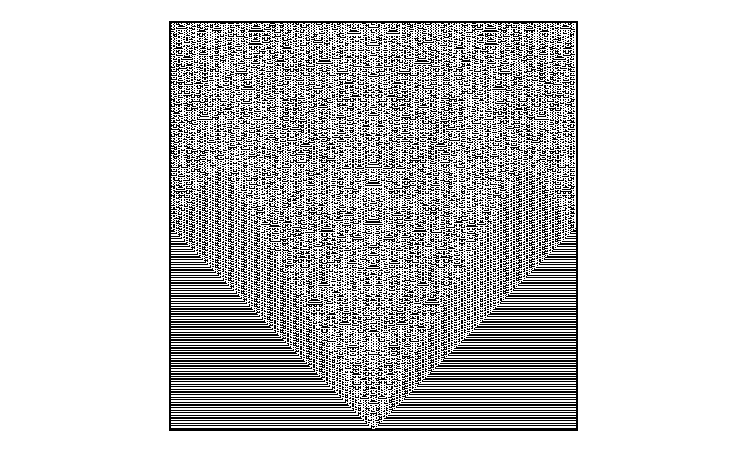
\includegraphics[trim = 40mm 0mm 0mm 0mm, width=1.7\textwidth]{./img/73_500}
 \caption{Rule 73}
\end{figure}


\begin{figure}
 \centering
 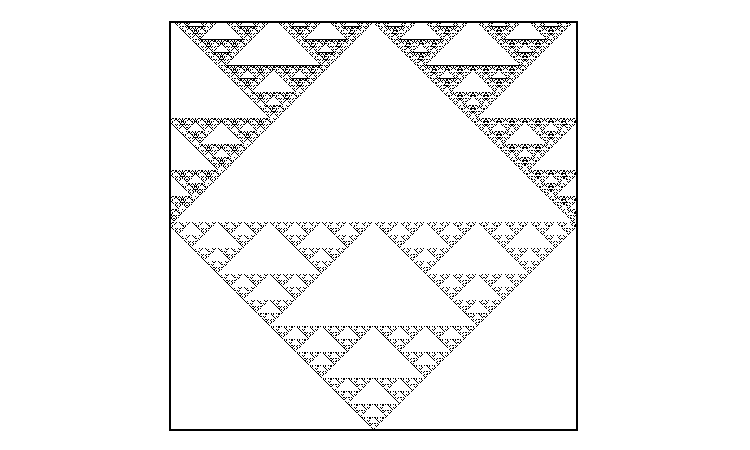
\includegraphics[trim = 40mm 0mm 0mm 0mm, width=1.7\textwidth]{./img/90_500}
 \caption{Sierpinski carpet - rule 90}
 \label{koberec}
\end{figure}


\begin{figure}
 \centering
 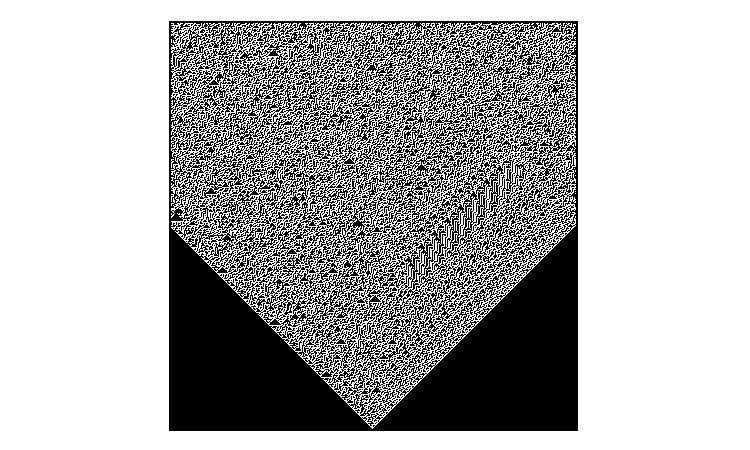
\includegraphics[trim = 40mm 0mm 0mm 0mm, width=1.7\textwidth]{./img/149_500}
 \caption{Rule 149}
 \label{koberec}
\end{figure}

\begin{figure}
 \centering
 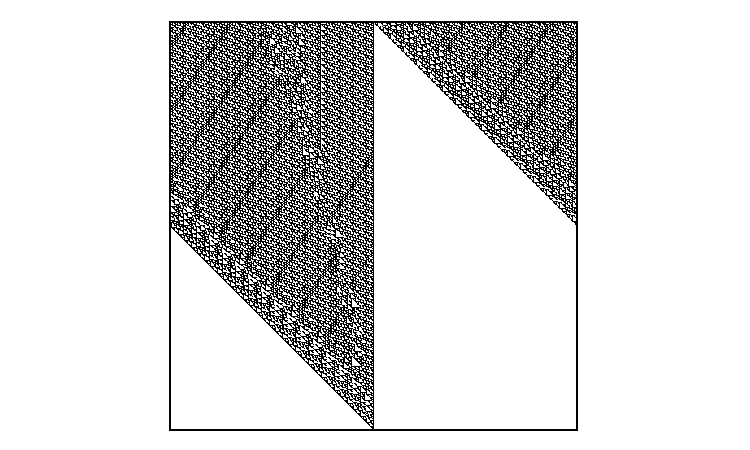
\includegraphics[trim = 40mm 0mm 0mm 0mm, width=1.7\textwidth]{./img/110_500}
 \caption{Rule 110}
\end{figure}

\begin{figure}
 \centering
 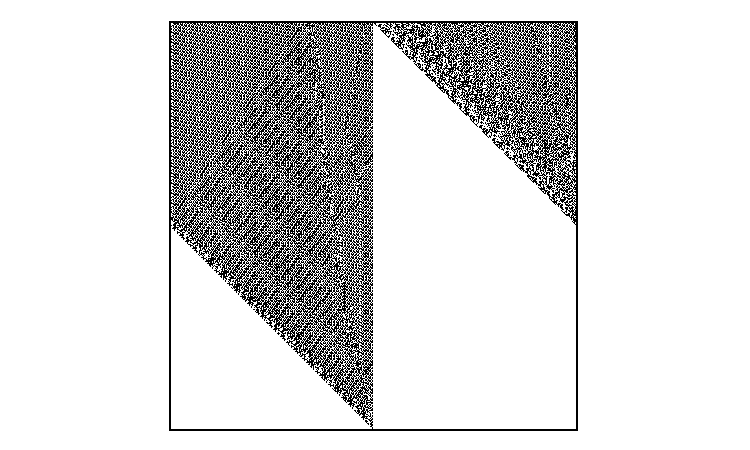
\includegraphics[trim = 40mm 0mm 0mm 0mm, width=1.7\textwidth]{./img/110_2000}
 \caption{Rule 110 -- $2000 \cross 2000$}
\end{figure}


\section{Rule 110}
The rule 110 is special among them. Cook have proved \cite{cook} that this rule is equivalent to the Turing machine, so depending on the initial conditions, it could be classified in any of the mentioned classes.

%First picture~\ref{koberec} is famous fractal known as Sierpinski carpet. Wolfram classified these 1D automata into four classes, based on the regularity of the pattern obtained.

%Wolfram argues that variety of behavior seen even in these most simple CA rises suspitions, and encourage hope, that in the infinitely large world of possible CAs, there is CA that model any complex phenomena you can imagine.


In his visionary book New kind of Science \cite{wolf}, Wolfram suggest possibility, that in the infinitely large world of cellular automata, there is an automaton that constitute a unified theory of the fundamental physics.
Although the details of his idea met with rejection(see \cite{aaronson}),
many notable physicists are attempting to construct such cellular automaton \cite{hooft}).
%
%Some of the basic construction principles for such automata are relevant also for our models, but mostly, we would diverge too far by further exploration.
%However, in the field of computational physics, cellular automata have already recorded success. And the focus of our 

However, focus of our work is much more modest that cellular automata describing universe.
Our focus is on the cellular automata that model flows of the fluids.

There is already a formal similarity between cellular automata we presented, and discrete partial differential equations. Consider the diffusion equation
\begin{align*}
\frac{\pd C}{\pd t} = \kappa \frac{\pd^2 C}{\pd x^2}.
\end{align*}
By discretization forward in time, it is transformed to
\begin{align*}
C_i^{(t)} = f\big[\sum_{j=-1}^{j=1}\alpha_j \, C_{i+j}^{(t-1)} \big]
\end{align*}
Formally, this equation corresponds to the rule of the one dimensional cellular automaton \ref{rule1}. However, $C_i$ is not from discrete finite set, but it is a continuous value, the $\alpha_i$ are not integers, but reals, and this would cause instability of this cellular automaton, as discussed in \cite{wolf} and the formal similarity leads to the dead end.

The connection of the cellular automata with the fluid mechanics is not straight-forward or formal, but it is grounded in the symmetries and conservation laws found in the hydrodynamic equations and the special class of cellular automata - the lattice gas cellular automata.

In these symmetries lies not only beauty of this method and their attractiveness for physicists, but their principal advantage over the better-established CFD methods.